\subsection{Onda completa con derivación central}
Este rectificador utiliza dos diodos \textbf{1N4007} conectados a un
transformador con derivación central y una resistencia de $10[\text{k}\Omega]$
que cumple la función de carga, como se muestra en la
\textbf{figura~\ref{circuito03}}, los voltajes entre las terminales del
transformador son iguales en magnitud, pero con diferentes fases.

\begin{figure}[!h]
\centering
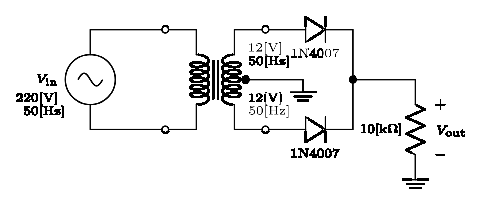
\includegraphics[scale=1.1]{diagramas/03.derivacion_central1.eps}
\caption{Rectificador de onda completa con transformador de derivación central.}
\label{circuito03}
\end{figure}

La polarización directa e inversa son alternadas en cada diodo del circuito por
lo que se obtienen solo los valores positivos de cada extremo del transformador.

\subsubsection{Simulación}
Se utilizó el software \emph{Quite Universal Circuit Simulator.} versión 23.3.1
para la simulación del rectificador de onda completa, este puede verse en la
\textbf{figura~\ref{simulacion03}}.

\begin{figure}[!h]
\centering
\includegraphics[scale=0.75]{simulacion/03.derivacion_central1.eps}
\caption{Simulación del rectificador de onda completa con derivación central.}
\label{simulacion03}
\end{figure}

\subsubsection{Laboratorio}
Se presenta el rectificador de onda completa con el transformador de derivación
central armado en laboratorio y su medición de voltaje de salida en la carga, en
la \textbf{figura~\ref{laboratorio05}}.

\begin{figure}[!h]
\centering
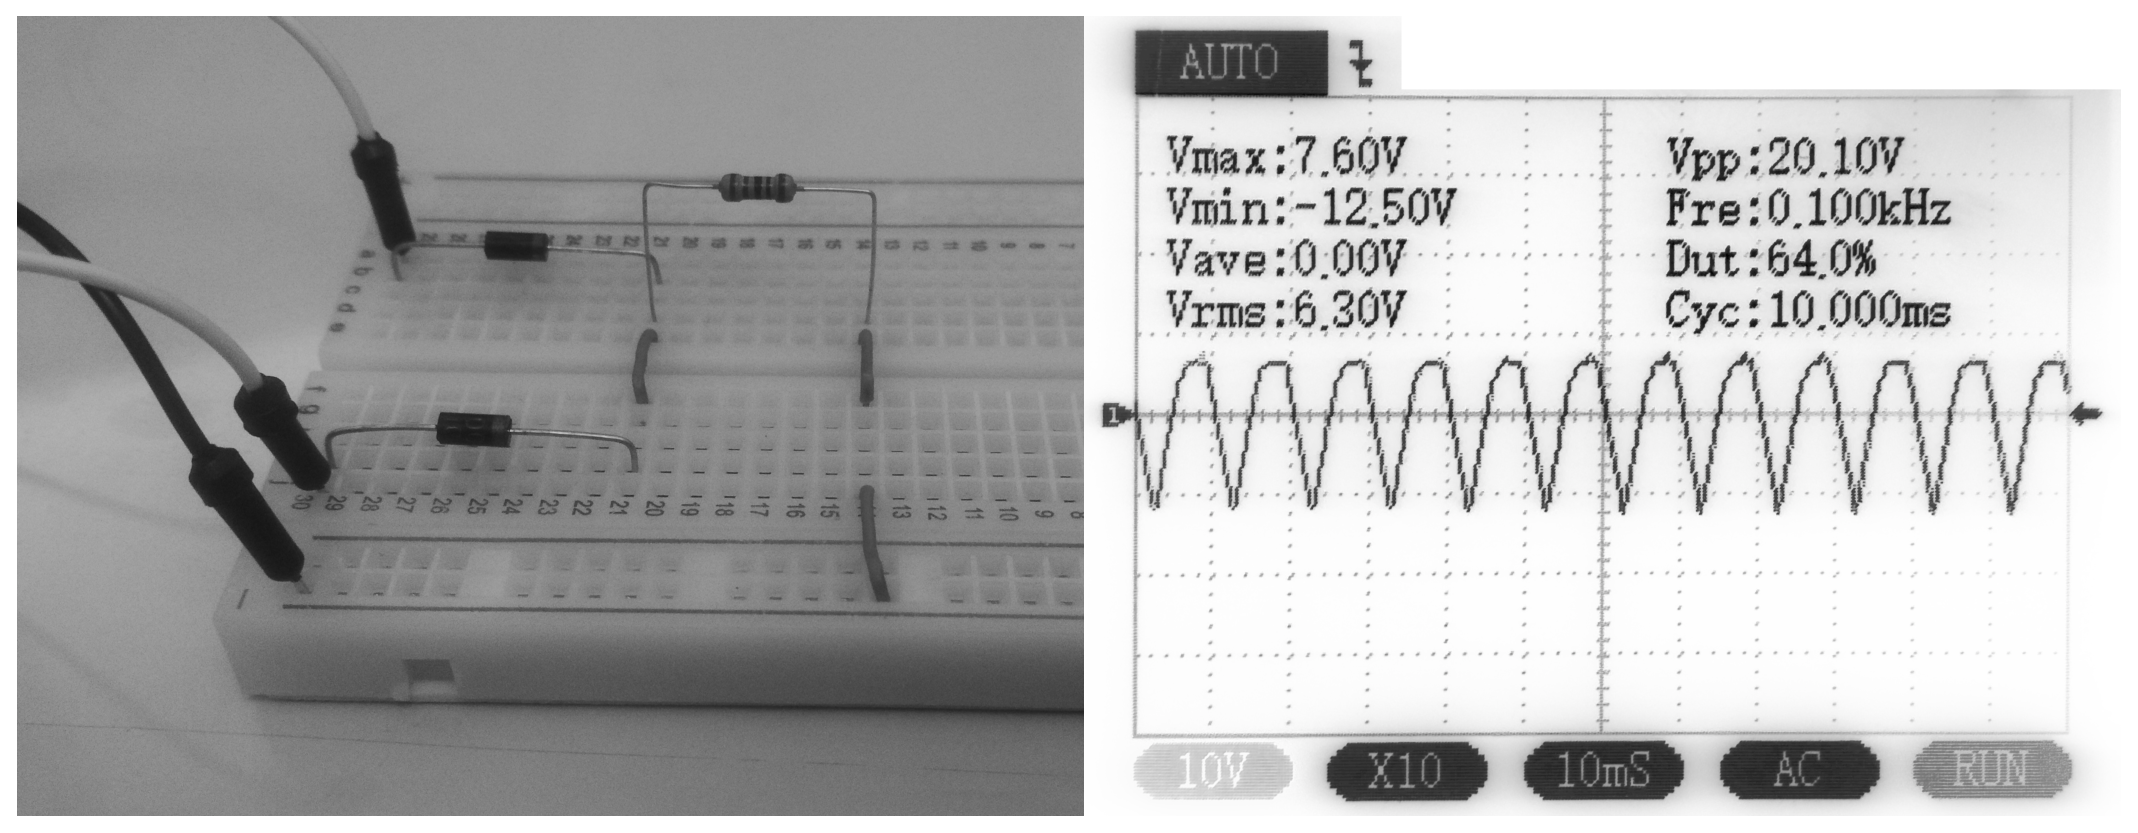
\includegraphics[scale=0.34]{fotos/03.derivacion_central1.eps}
\caption{Rectificador de onda completa con derivación central.}
\label{laboratorio05}
\end{figure}

